\opsim~and \altsched~schedulers have adopted two different ways of observing the sky. While the former relies on a greedy algorithm to decide which pointing should be performed (optimisation based on slew-time minimisation, optimal observing conditions - in terms of sky brightness and airmass for instance), the latter scans at the meridian dense areas (pre-defined at the begining of the night) of the sky. Figure xx illustrate the area observed at the end of a night for both schedulers.


\begin{figure}
  \centering
  \subfigure[OpSim]{\label{fig:opsim_night}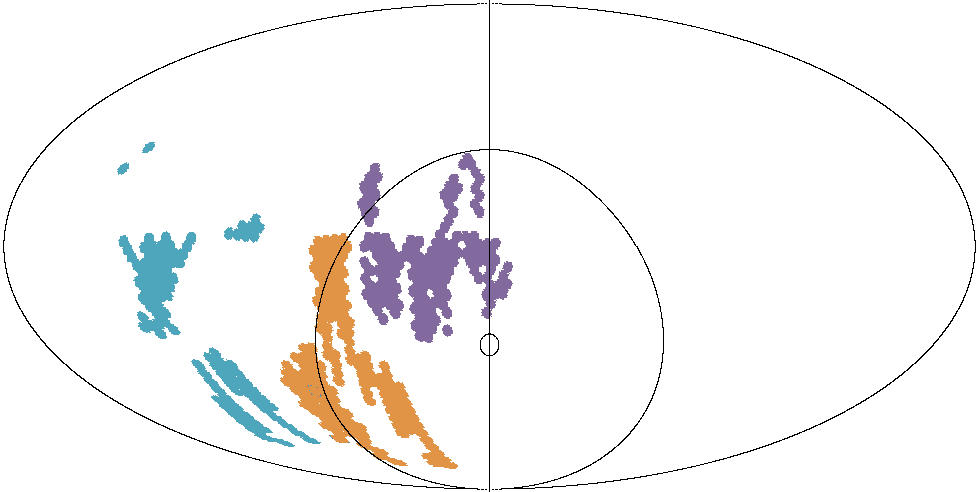
\includegraphics[width=0.8\textwidth]{opsim_vs_altsched/opsim_night.png}}
  \subfigure[altsched]{\label{fig:altsched_night}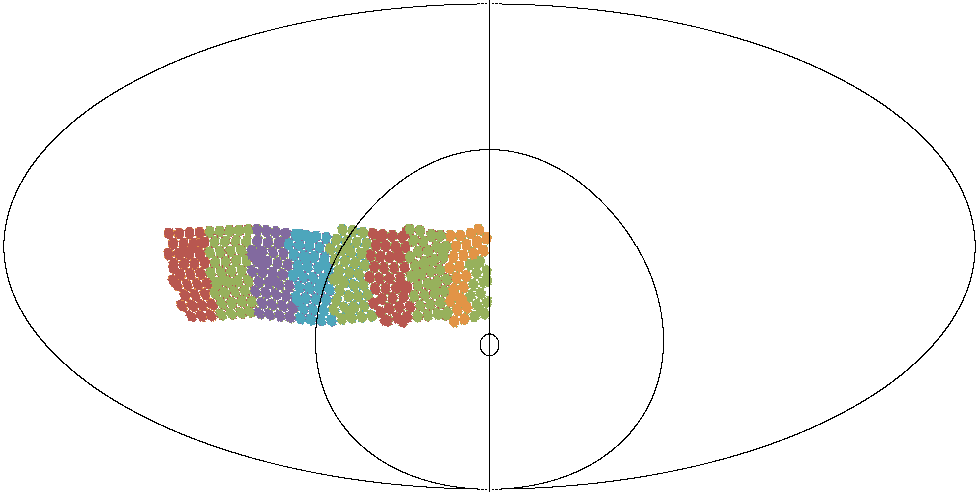
\includegraphics[width=0.8\textwidth]{opsim_vs_altsched/altsched_night.png}}
  \caption{Comparison for the DDFY1 and DDFY10 ROC curves}\label{fig:night_comp}
\end{figure}
